\section{Durchführung}
\label{sec:Durchführung}
Zur Bestimmung der Energiedifferenzen der Zeemann-Niveaus wird eine lichtdurchlässige Kammer, welche etwas Rubidium enthält, auf ca. $\SI{50}{\celsius}$ geheizt, sodass sich in ihr ein Gas aus Rubidiumatomen bildet. Diese werden durch eine Spektrallampe bestrahlt, aus deren Spektrum lediglich die D1-Linie mittels Filter gewählt wird. Zur Rechtszirkularpolarisierung des Lichtes werden zwei Polarisationsfilter, welche um $\SI{45}{\celsius}$ gegeneinander geneigt sind, verwandt.
\begin{figure}
  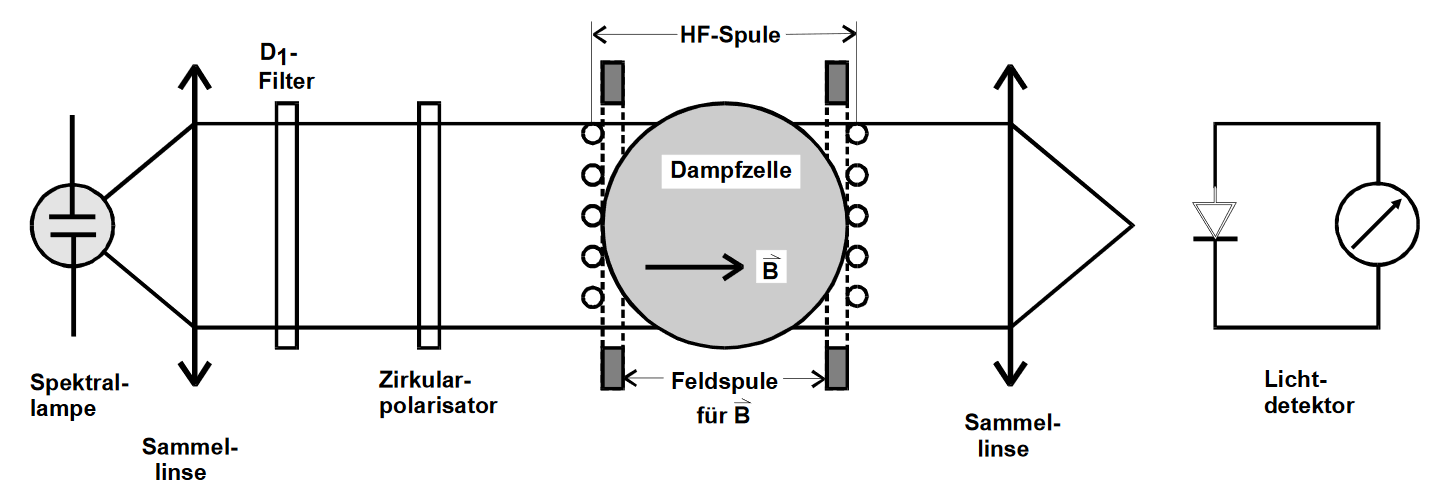
\includegraphics{./Aufbau.PNG}
  \caption{Schematische Darstellung der zur Messung verwandten Apparatur\cite{Anleitung}.}
  \label{fig:Aufbau}
\end{figure}
Nachdem das Licht die Probenkammer passiert hat, wird es auf einen Photodetektor zentriert, dessen Ausgangssignal an ein Oszilloskop geleitet wird.
Da zum optischen Pumpen eine Zeemann-Aufspaltung der Energieniveaus von Nöten ist und diese durch ein Magnetfeld hervorgerufen wird, muss das Erdmagnetfeld bestmöglich kompenisert werden. Hierzu wird der Strahlengang in Nord-Süd-Richtung gedreht, sodass die Horizontalfeldkomponente als konstante Verschiebung bei der Auswertung berechnet werden kann. Durch ein Helmholtzspulenpaar lässt sich ein Vertikalfeld aufbauen, welches die Vertikalfeldkomponente des Erdfeldes kompensiert. Hierzu wird auf dem Oszilloskop die an dem Photodetektor ankommende Intensität beobachtet und unter Zuhilfenahme eines Sweepgenerators entlang des Strahlenganges ein Magnetfeld kontinuierlich aufgebaut. Da bei $B=0$ keine Zeemann-Aufspaltung auftritt, kann kein optisches Pumpen angewandt werden, weshalb das Rubidiumgas einen Großteil des D1-Lichtes absorbiert und streut, weshalb die gemessene Intensität gering ist. Sobald ein Magnetfeld stark genug zur hinreichenden Niveauspaltung anliegt, wird gepumpt, weshalb die Atome kaum Photonen absorbieren können. Die Probe wird also transparent. Auf dem Oszilloskop ist so ein Anstieg der Intensität zu beobachten, welcher sich durch das Vertikalfeld sehr schmal einstellen lässt. Bei minimaler Breite des Anstiegs ist das Erdmagnetfeld bestmöglich kompensiert.
Nun Beginnt die Messung. Hierzu werden über eine Hochfrequenzspule Photonen der Frequenz $\nu$ quer durch die Probe gestrahlt, um diese im Photodetektor nicht zu messen. Diese Photonen sollen im Rubidium Übergänge innerhalb der Zeemann-Niveaus induzieren, weshalb durch die Sweepspule ein Magnetfeldbereich durchlaufen wird. Hierdurch werden die Zeemann-Niveaus solange auseinandergeschoben, bis $U_Z=h\nu$ gilt und induzierte Emission auftreten kann. Da die emittierten Photonen in alle Richtungen gestreut werden und nun wieder Elektronen in pumpbaren Zuständen vorliegen, wird erneut D1-Licht absorbiert und am Oszilloskop ist ein Einbruch der D1-Intensität zu sehen.
